\documentclass[a4paper]{article}

\usepackage[x11names]{xcolor}
\colorlet{bookcolor}{red!55!black}
\usepackage{tikz}

\begin{document}

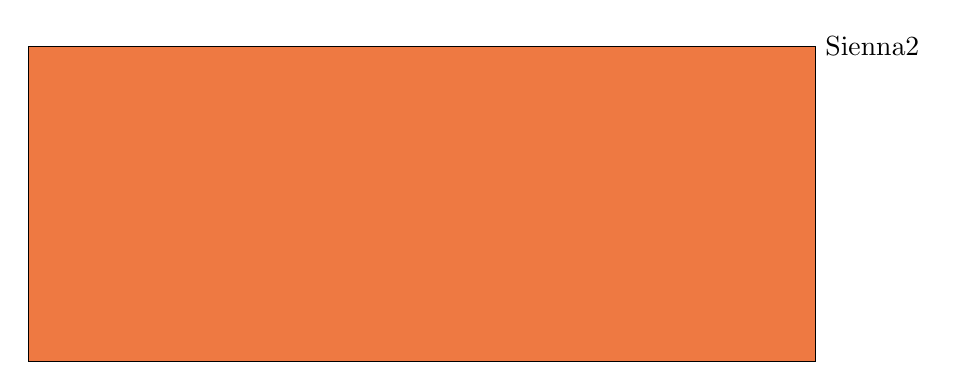
\begin{tikzpicture}
\draw[fill=Sienna2] (0,0) rectangle (10,4) node[right] {Sienna2};
\end{tikzpicture}


\begin{tikzpicture}
\draw[fill=bookcolor] (0,0) rectangle (10,4) node[right] {red!55!black};
\end{tikzpicture}

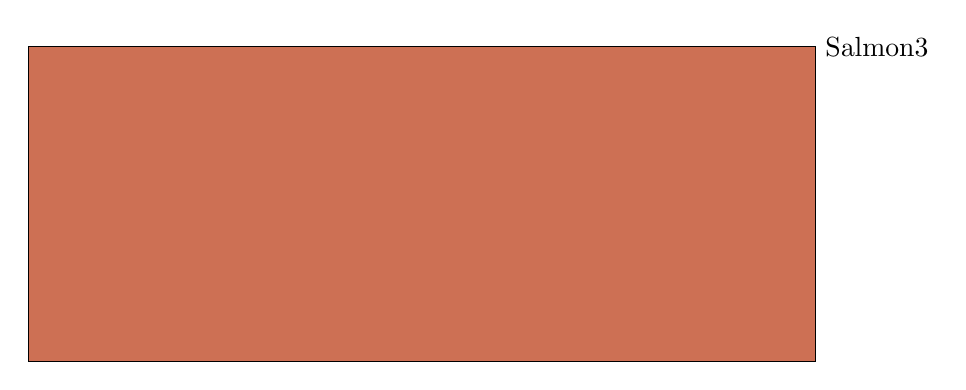
\begin{tikzpicture}
\draw[fill=Salmon3] (0,0) rectangle (10,4) node[right] {Salmon3};;
\end{tikzpicture}

\end{document}